\section{Introduction}
\label{sec:intro}

Multi-panel story image generation asks for a coherent visual sequence from a short narrative written as ordered scene blocks.
Unlike isolated text-to-image synthesis, each panel must be \emph{locally correct}---depicting the intended action and setting---and \emph{globally consistent}---keeping recurring characters recognizable across panels.
This dual requirement is difficult because independent per-scene generation often drifts in appearance, pronouns such as ``she'' or ``they'' must be mapped to the right subjects, and two-character scenes suffer from identity swapping or subject merging when a single visual anchor is forced onto both faces.

Our project builds a fully automated pipeline that separates textual story understanding from visual identity control.
An LLM-assisted planner produces strict structured metadata for characters and scenes; deterministic local code validates the plan, builds prompts, routes generation, and logs every decision.
The \textbf{submitted system} is a \emph{subject-count hybrid router}: stories with one distinct tagged entity use anchor-conditioned SDXL generation~\cite{podell2023sdxl} with IP-Adapter~\cite{ye2023ip-adapter}; stories with two or more entities use native ~\cite{zhou2024storydiffusion}, where front-loaded identity prompts initialize an internal identity bank.
This design follows a safety principle---single-anchor conditioning is skipped when two characters are equally important, rather than guessing one identity target.

 We also explored transformer-based diffusion method (PixArt-$\alpha$~\cite{chen2023pixartalpha}) with story-level cross-scene attention and DreamBooth LoRA~\cite{ruiz2022dreambooth}, as suggested for stronger long-range consistency.
That line is fully implemented and evaluated, but qualitative results remain below our hybrid baseline; we report it as an exploratory extension with explicit failure analysis.

\paragraph{Contributions.}
\begin{itemize}
  \item A reproducible structured prompt and identity framework spanning humans, animals, and robots, with subject-type-aware normalization.
  \item A subject-count hybrid generation policy combining IP-Adapter + SDXL for single-character stories and native StoryDiffusion for multi-character stories.
  \item Scene-consistency prompt assembly and CLIP-based~\cite{radford2021learning} panel selection for the single-character path.
  \item An exploratory PixArt-$\alpha$ DiT backend with LoRA and cross-scene blending, documented as a controlled negative comparison.
\end{itemize}

\begin{figure*}[!t]
  \centering
  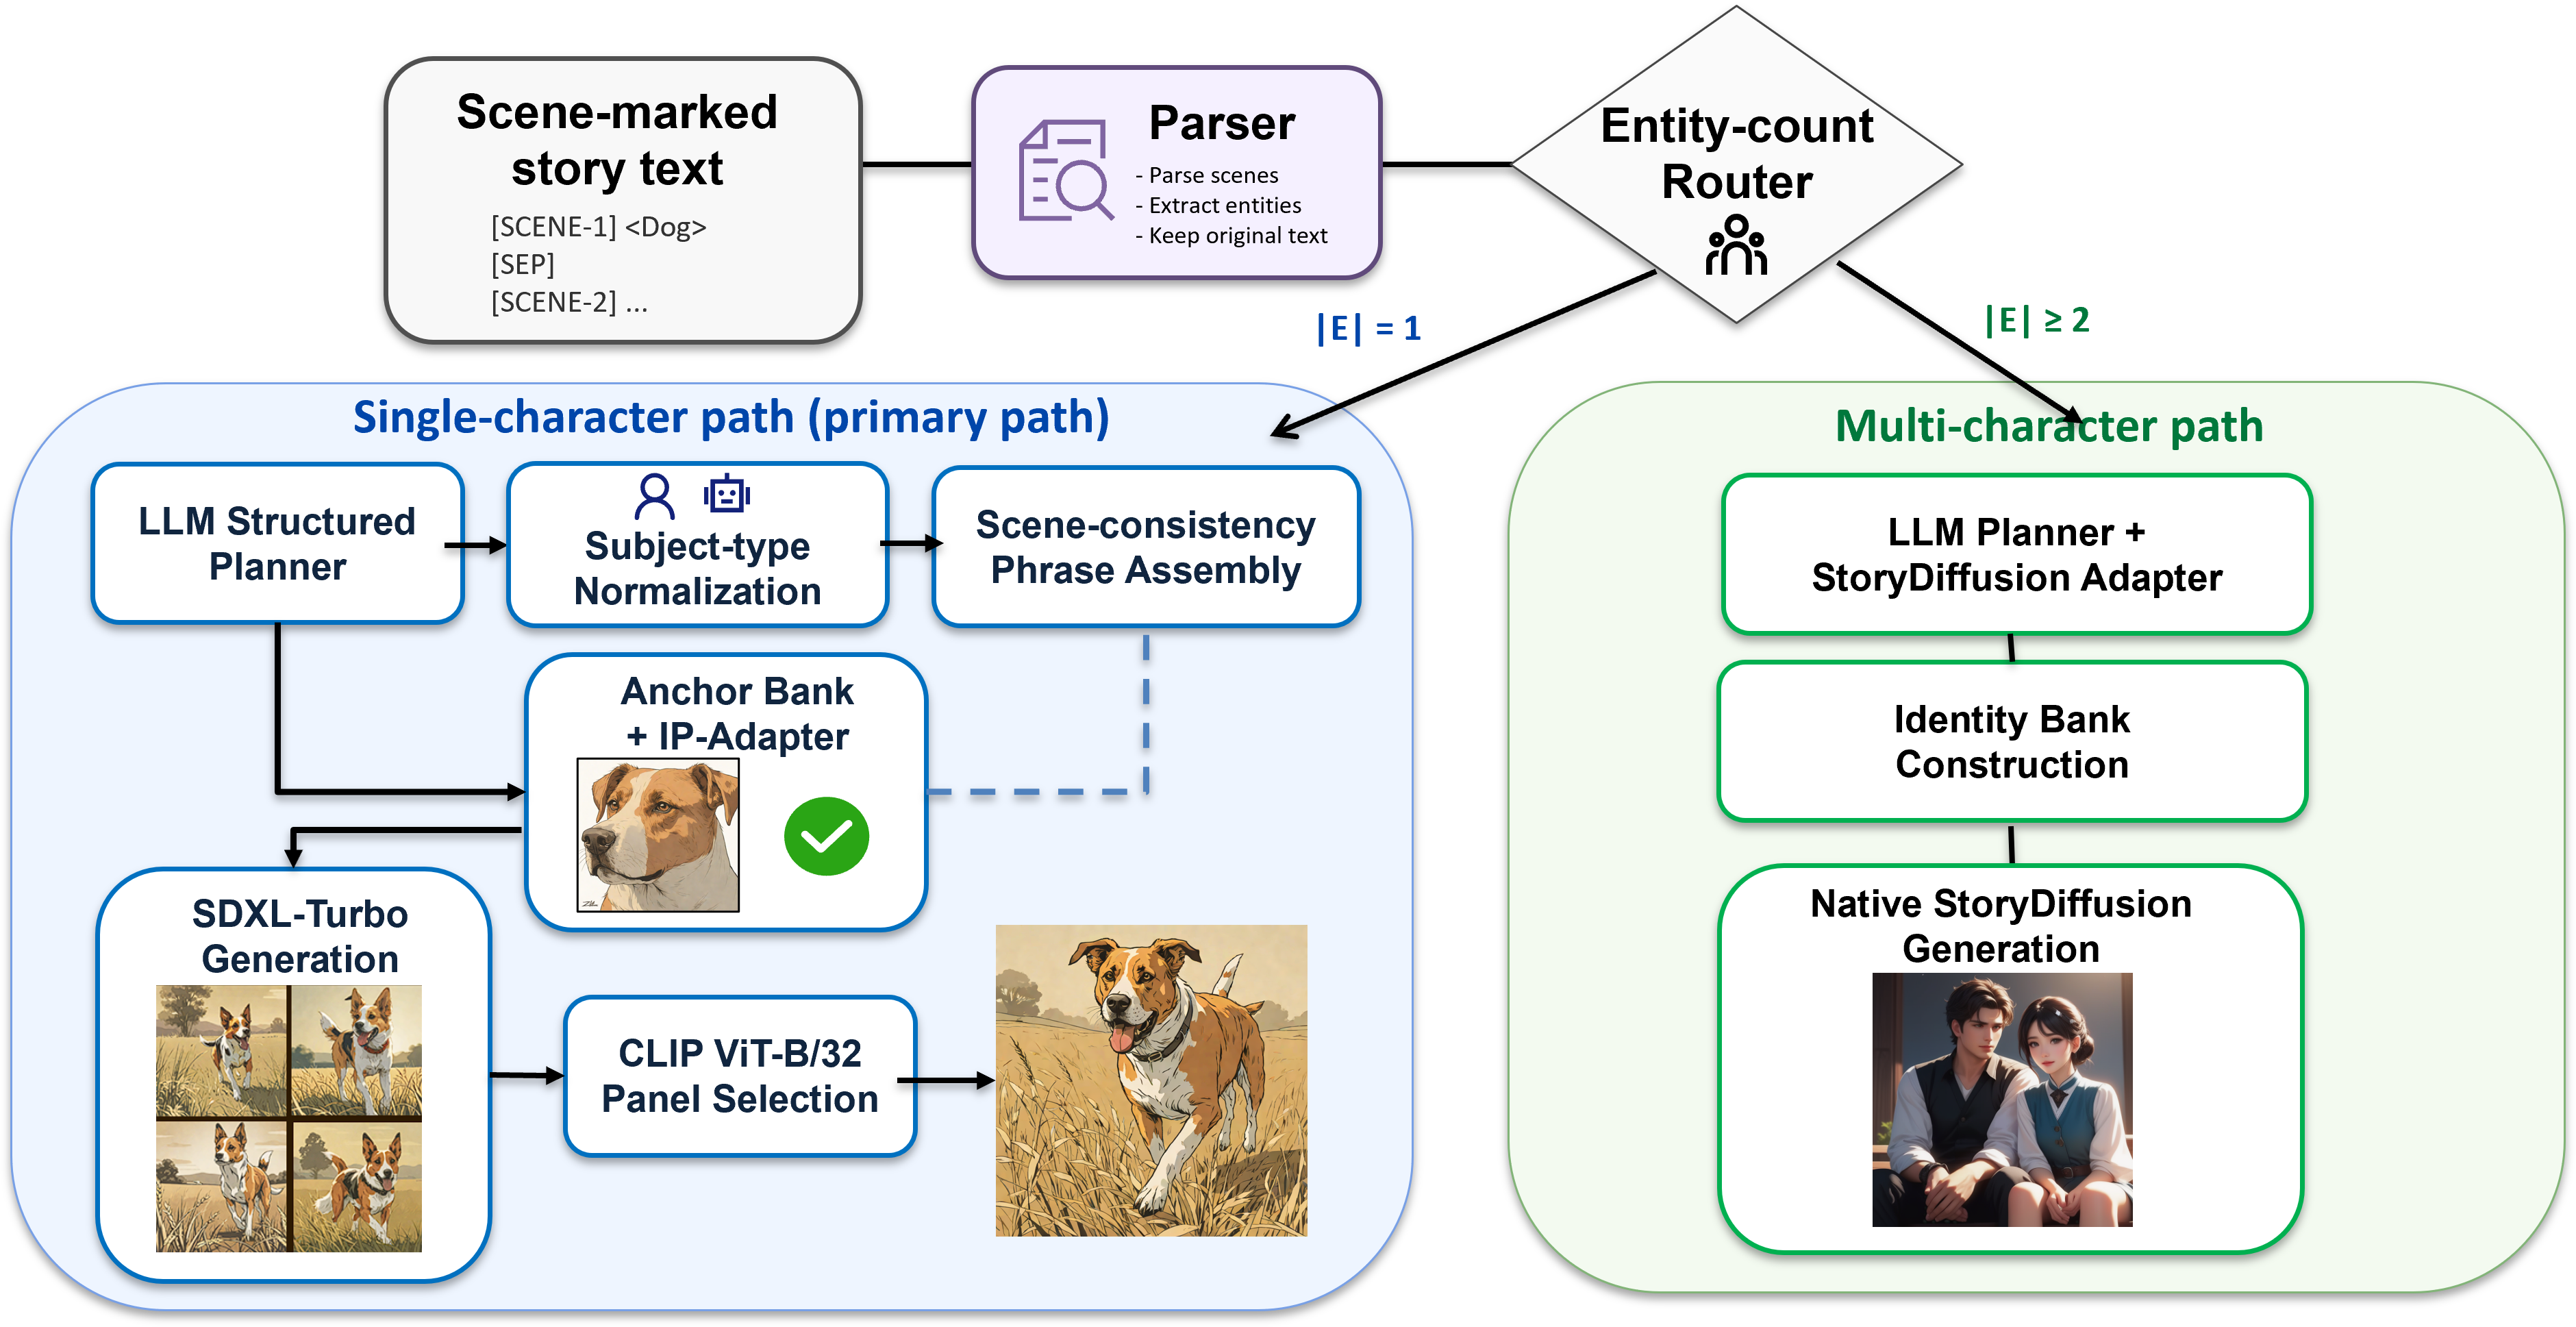
\includegraphics[width=\textwidth]{figs/pipeline.png}
  \caption{
  Overview of the proposed Subject-Count Hybrid Pipeline for multi-panel story image generation.
  The system first parses scene-marked story text and extracts structured character and scene metadata through an LLM-assisted planner.
  A subject-count router then dispatches the story to different generation backends:
  single-character stories use an anchor-conditioned SDXL + IP-Adapter pipeline with CLIP-based panel selection,
  while multi-character stories use native StoryDiffusion with identity-aware prompt adaptation.
  }
  \label{fig:pipeline}
\end{figure*}
